Advances in processor efficiency along with the development of energy-harvesting systems has created a new category of devices that require neither a battery nor a tethered power supply~\cite{prasad_comst_2014,lucia_snapl_2017,soyata_csm_2016}. These devices operate using ambient energy, such as radio frequency transmissions~\cite{rf_powered_computing_gollakota_2014}, light~\cite{margolies_infocom_2016,margolies_tosn_2016}, and vibration~\cite{gorlatova_sigmetrics_2014}. Incorporating compute, storage, sensing, and communication hardware~\cite{wisp5,moo}, such devices are a promising technology for use in the Internet of Things~\cite{ku_cst_2016}, in-body~\cite{nadeau_naturebio_2017} and on-body~\cite{bandodkar_electroanalysis_2015} medical systems, and energy-harvesting nano-satellites~\cite{kicksat}.

Energy-harvesting devices create unique challenges because they operate {\em intermittently} when energy is available~\cite{hicks_isca_2017,lucia_snapl_2017}. An
energy-harvesting device buffers energy in a small storage, e.g. a capacitor~\cite{gorlatova_tmc_2013},~\cite{gunduz_commag_2014} and when a threshold amount of energy accumulates, begins operating. Harvestable energy sources are low-power compared to a platform's operating level. A device operates briefly and when buffered energy is depleted, shuts down and recharges to operate again later. As an example, recharge time may be tens of seconds in radio frequency powered medical device~\cite[Fig. 3c]{nadeau_naturebio_2017}. Moreover, charge and discharge times vary by device (due to different capacitor sizes) and some may fail $\approx$10 to $\approx$100 times per second~\cite{tan_infocom_2016},~\cite{mementos},~\cite{nvp}.

%\begin{figure}
%	\begin{subfigure}[t]{.35\linewidth}
%		\centering\large Figure
%		\caption{\centering WISP~\cite{wisp} against an RFID antenna}\label{fig:1a}
%	\end{subfigure}%
%	\begin{subfigure}[t]{.65\linewidth}
%		\centering\large Figure
%		\caption{\centering Program X~\cite{hicks_mibench2_2016} (split into X and Y tasks~\cite{chain}) at two distances}\label{fig:1b}
%    \end{subfigure}
%	\caption{Impact of an inadequate task sizing on the computation speed of a moving transiently-powered device.}\label{fig:1}
%\end{figure}

\begin{figure}
	%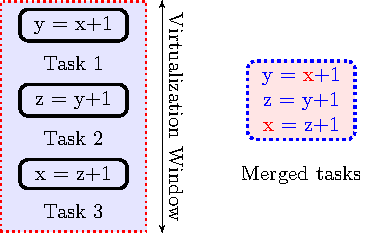
\includegraphics[width=.5\columnwidth]{presentation/images/alpaca-war.pdf}
    \caption{\label{fig:coalesce}Task decomposition is required for
intermittent execution but task transitions introduce overhead.}
\end{figure}


\textbf{Data Consistency in Intermittent Computing.} Software in an energy-harvesting system operates in the {\em intermittent execution model}~\cite{dino,lucia_snapl_2017}, with execution interrupted by failure periods. When power fails, a device loses volatile state, i.e., registers, stack, SRAM, and retains its non-volatile state, i.e., FRAM, Flash. While capturing periodic checkpoints~\cite{mementos,quickrecall} and sleep scheduling~\cite{dewdrop,hibernus,hibernusplusplus} help preserve execution progress, failures can leave volatile and non-volatile state inconsistent, leading to unrecoverable failures~\cite{dino,edb}. 

There are two main approaches for dealing with data inconsistency for intermittently-powered devices: (i) \emph{programming and execution models}~\cite{dino,ratchet,chain,alpaca} and (ii) \emph{architectures}~\cite{hicks_isca_2017,idetic,nvp,tictpl}. New architectures require hardware changes and are inapplicable to today's systems~\cite{hicks_isca_2017,nvp}, therefore new programming models and compilers are more suitable (as of now). However, they have their own limitations that need to be addressed---the core one being \emph{inability to adapt} to changing energy conditions.

\textbf{Task Decomposition of Intermittent Programs.} Recently proposed {\em
task-based} programming and execution models~\cite{alpaca,chain} advocate for
static decomposition of a program (by a programmer) into a collection of tasks.
Tasks can include arbitrary computation and, upon completion, are guaranteed to
have executed {\em atomically}, despite arbitrarily-timed power failures.
The programmer explicitly expresses task-to-task control flow.
%, which may be conditionally input-dependent.
%
Figure~\ref{fig:decomp} illustrates how the decomposition into tasks affects
the time the application takes to complete.
%
Each task transition introduces the overhead of tracking and atomically
committing the modifications to non-volatile memory by the task, to maintain
consistency of program state.
%
Naively minimizing the number of task transitions, (i.e. the task count),
\emph{at compile time} risks creating a task that requires more energy than the
device can buffer in its storage capacitor.
%
Such a large task would fail to complete unless the environment provides
sufficient incoming energy to supplement the energy in the capacitor.
%
To eliminate this risk, the programmer (or the compiler) must decompose the
program conservatively into many small tasks, at the cost of higher task
transition overhead.

One approach to decrease the task count, without assumming a minimum level of
incoming power always available, is to predict task energy consumption and
choose a decomposition specific to the device capacitor size.
%
Howerver, statically predicting energy of arbitrary input-dependent code with
peripheral access is a problem without a general solution.
%
Furthermore, a static decomposition approach cannot produce decompositions
portable across devices with different storage capacitorss.
%
In this paper, we propose a \emph{dynamic} task decomposition approach, that
accepts any static decomposition and opportunistically \emph{coalesces} tasks
at runtime when there is sufficient energy.

%A key challenge is that the length of a software
%task's execution is \emph{limited by the fixed total amount of energy} that a
%device can buffer in hardware. A task's code is static, but the duration of its
%execution may be input-dependent and is difficult to predict. To illustrate
%this, we refer to Figure~\ref{fig:1} showing the execution time of two
%applications (the same application X, but divided into X and Y tasks as
%in~\cite{chain}) running on RFID antenna-powered Computational
%RFID~\cite{wisp,rf_powered_computing_gollakota_2014} at two device-to-antenna
%distances (near---stable energy supply/far---high energy intermittency). At
%short distance: execution will takes too long caused by runtime cost of
%marshalling excessively small tasks. At far distance: program \emph{might never
%execute} if task execution consumes more energy than the system can buffer.
%This calls for at-runtime adaptive task division of any transiently-powered
%application---namely \emph{task virtualization}.

\textbf{Task Coalescing.} To add support for dynamic task
dvision to a task-based programming model, we propose a
\emph{task coalescing} mechanism: merging of atomic tasks
into a single (larger) task while preserving atomicity.
Merging two atomic tasks might produce a non-atomic task,
that may leave memory inconsistent after a partial
execution. A merge breaks atomicity when the accesses to
non-volatile memory from the previously atomic merged tasks
form a \emph{write-after-read (WAR)} dependency.
%
%variables in non-volatile memory at \emph{run-time} that can
%break the atomicity of the \emph{virtual task}. Consider the
%example depicted in Fig.~\ref{fig:virtualization}: Tasks 1,
%2 and 3 being executed consecutively. All tasks in this
%example are atomic since they do not have WAR dependency on
%the persistent variables they are accessing, e.g. \emph{x}
%is only read and \emph{y} is only written within Task 1.
%Now, suppose three tasks have been virtualized into a single
%one at run-time, namely Task 4: since \emph{x} is now first
%\emph{read} and then \emph{written}, a WAR dependency on
%\emph{x} is introduced dynamically at
%run-time---unfortunately Task 4 is \emph{no more atomic}
%since its re-execution will not always produce the same
%results.
%
Although WAR dependencies introduced by the \emph{static}
task division can be eliminated at compile time~\cite{alpaca}, those introduced \emph{dynamically} at
run-time cannot.
%
To maintain memory consistency in merged tasks, we propose a
mechanism for \emph{memory virtualization} that buffers the
updates to non-volatile variables in volatile memory before
committing them at the dynamic task boundary.
%
%Therefore, we require a \emph{new execution
%model} that keeps each virtual task atomic by committing the
%modified persistent variables at the boundary defined
%dynamically at run-time---keeping the non-volatile memory
%unmodified upon a power-interrupt and preserving its
%consistency.
%

Task coallescing removes the optimization burden of choosing
the best task decomposition from the programmer, because it
accepts any decomposition and improves it dynamically.
%
To further reduce the programmer effort, we propose a
compiler pass for \emph{automatic decomposition} of programs
into (small) \emph{atomic} tasks.
%
The compiler identifies non-volatile variables shared across
tasks as tasks are created, and instruments reads and writes
of those variables, using memory virtualization, to keep
the data consistent in the presence of power loss.
%
Despite being limited to a subset of the C language, the
automatic task decomposition allowed us to port several
applications to an intermittent platform with a moderate
effort.

We develop \sys%
\footnote{To be released at \url{http://anonymized.link}}
%
: a task coallescing system for task-based
programming models on intermittently-powered devices. The
capabilities required for effective coallescing mark our
contributions:

\begin{itemize}
\item Two adaptive coallescing strategies for selecting boundaries to coallesce based on past execution behavior
\item Software memory virtualization for transiently-powered devices that preserves atomicity of coallesced tasks
\item Compiler pass for automatic decomposition into small atomic tasks for adaptive coallescing at runtime
\end{itemize}


%Existing programming and execution models may require more accesses to non-volatile memory (for multi-versioning)~\cite{dino,chain} or may preclude the use of volatile memory~\cite{ratchet}. Effective use of both volatile and non-volatile memory is important for \emph{efficiency}, because non-volatile memory has higher access energy and latency than SRAM~\cite{nvp}, and \emph{generality}, because devices often have much more FRAM than SRAM (e.g., 64 times more in~\cite{wolverine}). How to connect this trade-off with task virtualization remains an open question.

%\textbf{Research Question and Contributions:} Specifically, we ask (i) how to use software support to \emph{dynamically adapt} the effective size of a task, while respecting programmer-specified task atomicity, and (ii) how to minimize run time and energy consumption while \emph{automatically maintaining memory consistency} during execution?

%To address this question, we develop {\bf \sys}: a new programming and execution model efficiently executing tasks which avoids non-termination across a range of energy buffer sizes, without burdening the programmer\footnote{Code will be available via \href{http://anonymized.link}{http://anonymized.link}.}. To accomplish this, \sys introduces two new capabilities: 

%\begin{itemize}
%	\item {\bf Dynamic task coalescing:} \sys's task coalescing mechanism dynamically executes multiple tasks as a single task. A programmer or compiler can specify small tasks that will execute on a device with a small energy buffer. Coalescing tasks allows running the same tasks on a device with a larger energy buffer, avoiding run time overheads associated with ending one task and beginning another.
%	%
%	\item {\bf Volatile memory virtualization with transiently-powered device:} Colascing through task virtualization requires memory virtualization. \sys's uses SRAM as working memory, which \sys dynamically populates with pages of data from FRAM on demand, during a task's execution. When a task ends, \sys commits dirty pages to FRAM using DMA block copies, ensuring task atomicity and memory consistency. To the best of our knowledge this is the first time when memory virtualization has been demonstrated on a transient power budget.
%\end{itemize}

We evaluated \sys end-to-end on a real energy-harvesting
device~\cite{wisp} running existing benchmarks ~\cite{chain}
and new programs. A comparison to a state-of-the-art
task-based system~\cite{chain} showed that \sys recovers
performance on conservative task decompositions missed by
systems with static decomposition.
%
%and can flexibly target a variety of platforms without rewriting code.
%
\todo{Provide concrete numeric results supporting this claim}{Amjad/Przemek}

%In this work we also address the problem of task construction burden imposed on the programmer. That is, we introduce \sys's compiler that transforms arbitrary C code into a graph of tasks that reflects the original program's control- and data-flow constraints. The compiler identifies data shared by multiple of the newly created tasks and instruments reads and writes of those data so that \sys's memory virtualization mechanism keeps those data consistent. While \sys's complier is still \emph{limited in scope}, e.g. is unable to handle instruction jumps, normalized loops and recursions, it already eliminates the labour-intensive process of writing tasks~\cite{chain,alpaca}, i.e., hours of programmer time.

%\sys's core contribution is the introduction of dynamic task coalescing mechanism. It allows the programmer or a compiler to intuitively decompose the program into small tasks that amortize fixed per-task overheads, yet present no risk of exceeding device energy capacity. As such a decomposition executes, \sys~{\em coalesces dynamically} consecutive tasks. Coalescing elides the commits of coalesced tasks by buffering multiple tasks' updates in an FRAM commit buffer. Periodically, as the span of the coalesced task grows, \sys ends coalescing and commits the state of the coalesced task. If a power failure interrupts a sequence of coalesced tasks, \sys adaptively reduces the number of tasks in that sequence that it will coalesce, committing sooner in future executions. Consequently, \sys's coalescing mechanism allows a program to execute efficiently across a range of energy buffer sizes, avoiding transition overheads in larger buffers, and ensuring progress in smaller buffers.

%We propose and explore two data swapping strategies for intermittently-powered systems based on FRAM/SRAM architecture. The first strategy is {\em demand paging}, which swaps the SRAM page with a new page from FRAM, buffering the swapped-out page until commit. The second strategy is {\em buffered direct access}, which directly reads and writes FRAM relying on dynamic double-buffering to ensure memory is consistent at commit.
